%% Section 5: Simulation methodology
\section{Simulation Methodology}
\label{sec:method}

\subsection{Models and parameters}
All models were built in MATLAB/Simulink with the Simscape Electrical (Powergui) continuous solver. Each model contains a DC source with series resistance $R_{dc}=0.049\;\Omega$ and a DC-link capacitor $C_{dc}=0.94$~F (as simulated), the bridge, the HERIC bypass where applicable, an L filter with $L_1=L_2=L$, a resistive load $R_L$ with its lower terminal grounded, and a parasitic capacitance $\Cpv=150$~nF between the negative DC rail and ground (Fig.~\ref{fig:model}). The value of $\Cpv$ lies within the 50--150~nF/kW range commonly quoted for crystalline modules. The leakage current is the current through $\Cpv$, measured with a current sensor and reported as an RMS value. The load is resistive and the model contains no grid source, current controller or phase-locked loop; the grounded load terminal plays the role of the grounded grid neutral, which is the reference that defines the CM loop. Table~\ref{tab:params} lists the parameters of the four cases.

\begin{table*}[!t]
\renewcommand{\arraystretch}{1.2}
\caption{Simulation parameters of the four cases ($\Cpv=150$~nF, $C_{dc}=0.94$~F, $R_{dc}=0.049\;\Omega$ in all cases)}
\label{tab:params}
\centering
\footnotesize
\resizebox{\textwidth}{!}{%
\begin{tabular}{lccccccccc}
\toprule
Case & $\Vdc$ (V) & $L_1=L_2$ & $R_L$ ($\Omega$) & $X_L/R_L$$^{c}$ & Est.\ $P_o$ (kW)$^{a}$ & Sweep (kHz) & $\Leq$ (mH) & $\fres$ (kHz) & Switch model$^{b}$ \\
\midrule
H4, unipolar   & 220 & 90~mH & 50    & 1.13 & 0.5 & 1--25 & 45 & 1.94 & MOSFET \\
H4, bipolar    & 460 & 10~mH & 10    & 0.63 & 7.4 & 1--40 & 5  & 5.81 & IGBT \\
HERIC, unipolar & 220 & 10~mH & 10.68 & 0.59 & 1.7 & 5--30 & 5  & 5.81 & IGBT \\
HERIC, bipolar  & 220 & 10~mH & 10.68 & 0.59 & 1.7 & 5--35 & 5  & 5.81 & IGBT \\
\bottomrule
\end{tabular}}\\[2pt]
\begin{minipage}{0.97\textwidth}\footnotesize
$^{c}$Series reactance of $L_1+L_2$ at 50~Hz relative to $R_L$. $^{a}$Estimated from the fundamental amplitude of the output voltage in the FFT results and $R_L$; \todo{confirm with the actual measured output power}. $^{b}$As listed in the simulation records; \todo{confirm device models and their on-state/switching parameters for each case}.
\end{minipage}
\end{table*}

\begin{figure}[!t]
\centering
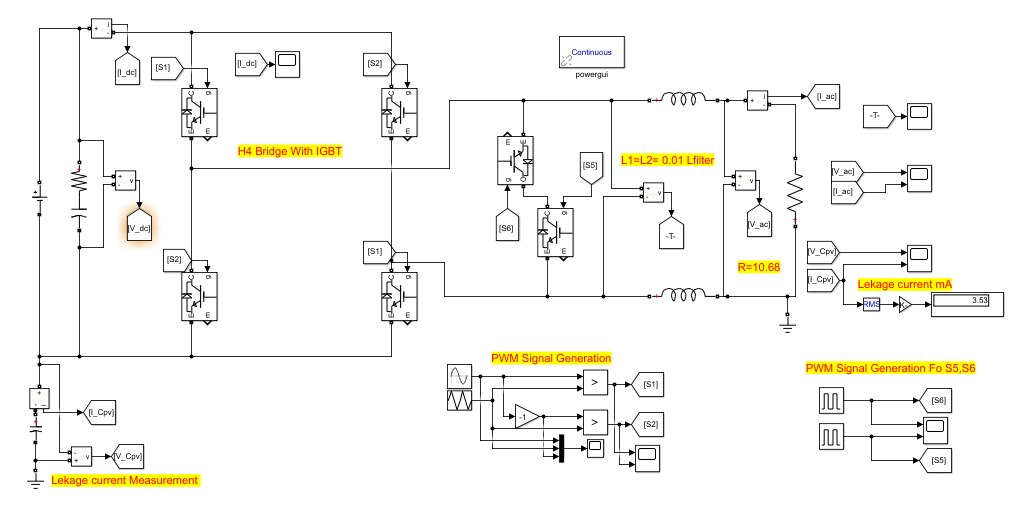
\includegraphics[width=\columnwidth]{figures/model_heric_bipolar.jpg}
\caption{Simulink model of the HERIC bipolar case. The H-bridge (IGBTs), the AC bypass ($S_5$, $S_6$), the L filter ($L_1=L_2=0.01$~H), the 10.68~$\Omega$ load with grounded lower terminal and the leakage-current measurement through $\Cpv$ are visible. The RMS leakage current is displayed in mA.}
\label{fig:model}
\end{figure}

The resonance frequencies in Table~\ref{tab:params} follow directly from~\eqref{eq:icm}: $\Leq=45$~mH gives $\fres=1.94$~kHz and $\Leq=5$~mH gives $\fres=5.81$~kHz.

\subsection{Metrics}
\emph{Leakage current:} RMS value of the current through $\Cpv$, compared with the 300~mA limit. \emph{Efficiency:} $\eta=P_o/P_{in}$ from the measured DC input and AC output powers; as the switch models include only their on-state and diode parameters, $\eta$ reflects conduction-type loss and does not constitute a complete switching-loss or thermal assessment. \emph{THD:} computed by the Powergui FFT tool on the load voltage (for a resistive load, voltage and current THD are identical), with the fundamental at 50~Hz. The tool was configured for harmonic orders up to the 40th (2~kHz); hence the reported THD is a \emph{low-order} THD that excludes the switching-frequency sidebands, which are attenuated by the filter and are addressed by the standards separately. Observation windows were 2--5 fundamental cycles after the start-up transient (stop time 0.05--0.08~s).

\subsection{Sweeps}
For each case the switching frequency was swept in steps of 0.5--1~kHz at low frequencies and in larger steps above 20~kHz, with the other parameters constant. The resulting resolution (0.5--1~kHz near the resonance) limits the accuracy with which the peak position can be located to about $\pm 0.5$~kHz.

\subsection{Study workflow and post-processing}
Fig.~\ref{fig:workflow} summarizes the procedure applied to each of the four cases. The analytical resonance $\fres$ was computed from \eqref{eq:fres} before the simulations were run, so that the comparison with the sweep results is a prediction and not a fit. For every switching frequency in the sweep, the model was run to the stop time of Table~\ref{tab:repro}, and three metrics were extracted from the last 2--5 fundamental cycles: the RMS value of the current through $\Cpv$, the efficiency from the DC input and AC output powers, and the low-order THD from the Powergui FFT tool. Leakage peaks were identified as local maxima of the leakage-versus-frequency curve in the sweep plots, and the deviation of a peak from the prediction was defined as the difference between the peak frequency and the nearest predicted frequency among $\fres$, $\fres/2$, $\fres/3$ and $2\fres$, relative to that predicted frequency (Table~\ref{tab:res}). The selection rule of Section~\ref{sec:design} was derived from these deviations and from the width of the observed peaks, and was not optimized against any additional data.

\begin{figure}[!t]
\centering
\begin{tikzpicture}[font=\footnotesize,node distance=4.5mm,
 blk/.style={draw,thick,rounded corners=2pt,minimum width=7.4cm,minimum height=6.5mm,align=center,fill=gray!8},
 arr/.style={-{Latex[length=2mm]},thick}]
\node[blk] (a) {1. Build model and set parameters of Table~\ref{tab:params} ($\Vdc$, $L$, $R_L$, $\Cpv$)};
\node[blk,below=of a] (b) {2. Compute $\Leq$ and $\fres=1/(2\pi\sqrt{\Leq\Cpv})$ \emph{before} simulating};
\node[blk,below=of b] (c) {3. For each $\fsw$ in the sweep, run the simulation to the stop time};
\node[blk,below=of c] (d) {4. Record RMS $\iCM$, efficiency and low-order THD (last 2--5 cycles)};
\node[blk,below=of d] (e) {5. Plot metrics versus $\fsw$; locate local maxima of $\iCM$};
\node[blk,below=of e] (f) {6. Compare $f_{\mathrm{peak}}$ with $\fres$, $\fres/k$, $2\fres$; compute deviation};
\node[blk,below=of f] (g) {7. State the selection rule and check the 300~mA limit};
\foreach \x/\y in {a/b,b/c,c/d,d/e,e/f,f/g} \draw[arr] (\x.south)--(\y.north);
\end{tikzpicture}
\caption{Study workflow applied to each of the four cases.}
\label{fig:workflow}
\end{figure}
